\section{Current Electricity}

\subsection{Circuit Board}
\begin{itemize}
\item{Preparation Time: 1 hour}
\item{Materials: Piece of flat wood, staples or small nails, hammer, broken radio case, glue, any circuit components}
\item{Procedure: Draw out a grid on the wood with squares about 5-6 cm on a side. At each grid intersection, gently tap in a staple or small nail. From the radio, take the battery casing with its terminals and clips and glue it to one side of the wood; this will be your power supply. Using any configuration you like, set up a circuit on the board using the pins as wire holders. This makes the circuit easier to handle and see.}
\end{itemize}

\subsection{Breadboards}
\begin{itemize}
\item{Preparation Time: 3-4 hours}
\item{Materials: shower sandal (new), knife, glue, sewing needle, metal strips or aluminum foil (0.5 - 1 cm wide, 5 - 10 cm long), sharpie or marker, simple circuit components}
\item{Construction: Remove the sole of the sandal and cut the bottom layer (about 0.5 cm; keep this piece whole for later) off the sandal. Inlay the metal strips at angles into the other section of the sandal in the arrangement shown below. These are the wires of your breadboard. The two long, thin sections are your power strips; the larger section is the board itself where circuit components will be placed. The angle of the metal strips allows the components to remain in contact with the strips under the constriction of the rubber sandal, but if another configuration works better, do that.\\
The diagram shows the layout of a typical breadboard; change this as necessary. Replace the cut-off section of sandal; you will need to cut slots for the metal strips to fit snugly. Using the sewing needle, punch thin holes into the bottom of the sandal along the lines of the metal strips, about 1 cm apart. Use a sharpie or marker to indicate the positions of the holes and the outlines of the different sections on the breadboard, as shown above. On the power strips, label one line as positive and the other as negative. Use glue to keep the pieces of sandal together. Now your breadboard is done; some modification may be necessary depending on the resources available.\\
As for electrical components, broken radios, cell phone chargers, old computers, etc., can be stripped for parts. Resistors, transistors, capacitors (parallel plate or cylindrical), diodes, variable resistors (rheostats), switches, fans, LEDs, heat syncs, speakers, and wires can be found easily, even in villages without electricity. If you are stuck, drop a few shillings at the Broken Stuff shop in town.}
\item{Procedure: Using your new broken radios, pull out the various components and place them in the breadboard as the circuit you desire. Connect the negative and positive ends of this circuit into the power strips, and the appropriate terminals of the power strips to some batteries, or an accumulator. If you smell burning resistors, that is another lesson. If not, then you have a circuit to play with.}
\item{Theory: Students spend plenty of time staring at circuit drawings on the board and sometimes become fairly adept at analyzing them, but when shown a real circuit they cannot tell parallel from series. When teaching simple circuits, accompany any real circuit with a drawing for students to follow.}
\end{itemize}


%Potential Difference and Emf

%Factors Determining Resistance

%Resistors (Wire coil, variable, fixed)

%Internal Resistance of a Cell / Wheatstone Bridge

\subsection{Construction of a Metre bridge and Potentiometer}

\subsubsection*{Learning Objectives}
\begin{itemize}
\item{To construct and use a metre bridge and potentiometer} 
\end{itemize}

\subsubsection*{Background Information}
A metre bridge can be used to determine the resistance of various conductors and also to compare the Emf of batteries. It consists of a piece of resistance wire 1 m long attached in series to either a rheostat or other conductors and resistors. By using a galvanometer we can find the length of resistance wire needed to equal the resistance of the other conductors. Or we can use a voltmeter to find the potential difference along a length of the resistance wire. There are several activities that can be done with a metre bridge and each requires different materials. The construction of the metre bridge itself, however, is the same, and follows below.

\subsubsection*{Materials}
Piece of wood 110 cm by 4 cm, shoe tacks or small nails or screws, connecting wire, Constantine or nichrome wire, dry cells, resistors of known and unknown resistance, galvanometer. Alternative: Voltmeter, rheostat, micrometer screw gauge

\subsubsection*{Hazards and Safety}
\begin{itemize}
\item{Make sure all nails are removed.} 
\end{itemize}

\subsubsection*{Preparation Procedure}
\begin{enumerate}
\item{From one side of the piece of wood, measure 5~cm and fix 2 shoe tacks or nails side by side about 2.5~cm apart, as shown in \ref{fig:metre-bridge}. From one of the nails measure 10~cm and fix another nail. Leave a space of about 6-8~cm and fix another nail. From the first nail again measure 50~cm and fix another nail.} 
\item{Again from the first nail measure 100~cm and fix two nails apart as with the first end. From this end on the side of one of the nails measure 10~cm and fix another nail, leave a gap and fix another nail.} 
\item{On the other long side place a meter ruler from first nail to the last nail, mark each cm and write the scale interval of 10~cm.} 
\item{Fix Constantine wire from the first nail to last nail along the side with the cm markings and make sure the wire is tight.} 
\end{enumerate}

\begin{figure}
\begin{center}
\def\svgwidth{350pt}
\input{./img/metre-bridge.pdf_tex}
\caption{A Metre Bridge}
\label{fig:metre-bridge}
\end{center}
\end{figure}

\subsubsection*{Activity Procedure}
\begin{enumerate}
\item{Use connecting wire to join one of the nails holding the resistance wire to the second nail along the side without the cm markings. Then leave a gap and connect another wire to the central nail and then to next nail. Leave another gap and connect a wire from following nail to nail holding the other end of the resistance wire.} 
\item{Connect a metre bridge circuit by connecting one known and one unknown resistor into each of the gaps.} 
\item{Connect one terminal of a galvanometer to the center nail of the metre bridge. Connect the other terminal to a connecting wire which can be moved easily along the resistance wire.} 
\item{Move the galvanometer wire along the resistance wire until the galvanometer reads zero; that is no current is flowing.} 
\item{Measure the length of resistance wire on both sides of the galvanometer wire. Call the left side of the metre bridge ``one'' and the right side ``two'' so these lengths are $L_1$ and $L_2$.} 
\item{Write these two lengths as a ratio, for example the length on the left side divided by the length on the right side, $\frac{L_1}{L_2}$.} 
\item{Set this ratio equal to the ratio of resistances of the resistors, in this case the resistor on the left divided by the resistor on the right (one of these resistances is know, one is not).
$$ \frac{L_1}{L_2} = \frac{R_1}{R_2} $$ 
}
\item{Solve this equation to find the resistance of the unknown resistor, that is $$ R_1 = R_2 \frac{L_1}{L_2} $$ $$\mathrm{OR}$$ $$ R_2 = R_1 \frac{L_2}{L_1} $$
} 
\end{enumerate}

\begin{figure}
\begin{center}
%\def\svgwidth{300pt}
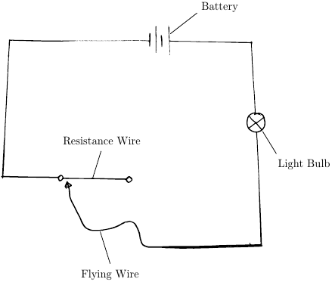
\includegraphics{./img/ohm's-law.png}
\caption{Metre bridge circuit}
\label{fig:ohm's-law}
\end{center}
\end{figure}

\subsubsection{Alternative Activity: Potentiometer}
\begin{enumerate}
\item{In the gaps of the metre bridge, place a rheostat, dry cells and a switch.} 
\item{Connect one terminal of a voltmeter to the nail holding the resistance wire at the 0 cm mark.} 
\item{Connect the other terminal of the voltmeter to a connecting wire which can easily move along the resistance wire.} 
\item{Close the switch so that current is moving through the circuit.} 
\item{Move the voltmeter wire to the 10 cm mark and read the voltage. This is the potential difference across 10 cm of the resistance wire.} 
\item{Move the voltmeter wire to the 20 cm mark and read the voltage. Repeat this process for 30, 40, 50, etc. cm and record all of the values.} 
\item{Use the callipers to measure the diameter of the wire.} 
\item{Make a graph of resistance and length. Use this graph to find the resistivity of the resistance wire.} 
\end{enumerate}

\begin{figure}
\begin{center}
\def\svgwidth{300pt}
\input{./img/potential-metre.pdf_tex}
\caption{Layout of a Potentiometer}
\label{fig:potential-metre}
\end{center}
\end{figure}

\subsubsection*{Results and Conclusions}
A constructed metre bridge functions using the relationship between a wire's length and its resistance. This principle can be used to find the resistivity of the wire or to find the resistance of any other conductors.  

\subsubsection*{Clean Up Procedure}
Remove any remaining nails, pieces of wood and other equipment.

\subsubsection*{Discussion Question}
How can you manufacture a potentiometer?

\subsubsection*{Notes}
Metre bridges are used to determine unknown resistance and to compare electromotive force.  When you are using a metre bridge to find the resistance of an unknown resistor, be sure to use two resistors that are similar in resistance. If the resistances are too different, it will be difficult to find with precision the point on the wire where the galvanometer reads zero.

This setup can also be used as a potential meter (potentiometer) in order to find the resistivity of the resistance wire.  

%Heating Effect of Electric Current (Joule’s Law)

\subsection{Making an Electric Heater}

\subsubsection*{Learning Objectives}
\begin{itemize}
\item{To prepare and demonstrate an electric heater} 
\end{itemize}

\subsubsection*{Background Information}
Electricity and heat are both forms of energy, so it is possible to change energy from one form to another.  

\subsubsection*{Materials}
1 m of resistance wire (nichrome) of swg 30 or 32, small piece of wood or paper, connecting wires, two to four dry cells (batteries), container of water, optional thermometer

\subsubsection*{Hazards and Safety}
\begin{itemize}
\item{If the heater is connected to the cells while not in the water, the wire can melt or burn other objects.} 
\end{itemize}

\subsubsection*{Preparation Procedure}
\begin{enumerate}
\item{Collect all materials.} 
\item{Cut a small piece of wood about 4 to 6 cm long, or roll a piece of paper.} 
\end{enumerate}

\subsubsection*{Activity Procedure}
\begin{enumerate}
\item{Coil the resistance wire onto the piece of wood or rolled paper so that the coils are close but not touching. Use the entire wire.} 
\item{Use connecting wires to connect the ends of the resistance wire to the terminals of the batteries.} 
\item{Place the coil of resistance wire into the container of water.} 
\item{Observe any effects on the water when current is flowing through the coil. Use your hand on the outside of the container to test the temperature.} 
\end{enumerate}

\begin{figure}[h]
\begin{center}
%\def\svgwidth{150pt}
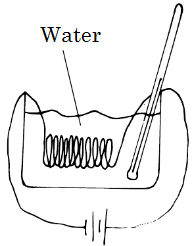
\includegraphics{./img/electric-heater.png}
\caption{An Electric Water Heater}
\label{fig:electric-heater}
\end{center}
\end{figure}

\subsubsection*{Results and Conclusions}
When the heater (coil) is left in the container of water for a few minutes, the temperature of the water rises enough that it can be felt by your hand on the outside of the container. If the heater is left for a long time, the water may boil.  

\subsubsection*{Clean Up Procedure}
\begin{enumerate}
\item{Remove the waste products and dry the water on the table.} 
\item{Return all materials to their proper places.} 
\end{enumerate}

\subsubsection*{Discussion Questions}
\begin{enumerate}
\item{What kind of energy is being produced?}
\item{What kind of energy is being converted?}
\end{enumerate}

\subsubsection*{Notes}
The electric heater converts electrical energy into heat energy. It can be used to boil water or other liquids, or to heat houses. The larger the coils are, the more efficient the heater will be.  

%Electrical Installation of a House (Fuse)

%\subsection{Foil Fuse}
%\begin{itemize}
%\item{Preparation Time: 15 minutes}
%\item{Materials: Power source, wires, two small nails, small piece of wood, metal foil (from Blueband container, gum, etc.)}
%\item{Procedure: Hammer the nails into the wood about 5 cm apart to act as wire terminals. Connect wires to each of the nails and place a thin strip of foil between the nails, bending it around the nails to secure it. Connect the wires to the power source. If the source is powerful enough, it will cause the foil to heat and eventually burn, breaking the circuit.}
%\item{Theory: Foil, having a very small cross-sectional area compared to that of a wire, has a low tolerance for current. If too much current passes through the foil, it will burn away. This is essentially how a fuse works in a radio or other electrical device. To be more scientific in your experiment, use a rheostat in the circuit, gradually lowering the rheostats resistance until the fuse blows.}
%\end{itemize}


\subsection{Fuse}

\subsubsection*{Learning Objectives}
\begin{itemize}
\item{To understand the effect of a strong electric current on a wire of high resistance}
\item{To understand the use of a fuse in electrical devices and installations}
\end{itemize}

\subsubsection*{Background Information}
When a strong current is passed through a wire of high resistance (depending on the material, area and length), some of the electrical energy is converted into heat energy.  If enough heat is produced, the wire burns and stops conducting electricity, breaking the circuit.  This device can be used to protect electrical devices like radios or computers from electrical surges.  If placed before all the components in a circuit, this thin wire, called a fuse, will break if too much current is passed through the circuit.

\subsubsection*{Materials}
Power source, wires, two small nails, small piece of wood, metal foil (from Blueband container, wrapper, etc.)

\subsubsection*{Preparation Procedure}
\begin{enumerate}
\item{Hammer the nails into the wood about 5 cm apart.}
\item{Connect wires to each of the nails.}
\item{Place a thin strip of foil between the nails, bending it around the nails to secure it.}
\end{enumerate}

\subsubsection*{Activity Procedure}
\begin{enumerate}
\item{Connect the wires to a power source to complete the circuit.}
\item{Observe the effect of the current on the foil when a large current is passing.}
\end{enumerate}

\subsubsection*{Results and Conclusions}
If the source is powerful enough, it will cause the foil to heat and eventually burn, breaking the circuit.  It will be seen that the circuit will work at first, but then the foil will burn.  Foil has a very small cross-sectional area compared to that of a wire, so it has a low tolerance for current. If too much current passes through the foil, it will burn away. This is essentially how a fuse works in a radio or other electrical device.

\subsubsection*{Cleanup Procedure}
\begin{enumerate}
\item{Disconnect the wires from the battery.}
\item{Dispose of the burnt fuse and return all materials to their proper places.}
\end{enumerate}

\subsubsection*{Discussion Questions}
\begin{enumerate}
\item{What causes the fuse to burn?}
\item{Why would a fuse be useful in an electrical device?}
\end{enumerate}

\subsubsection*{Notes}
It is best to use a rheostat in this circuit.  Begin with a high resistance on the rheostat; slowly decrease it so that the foil is taking more of the voltage.  As the voltage is increased, the foil will eventually burn as its resistance reaches a maximum.
You can ind fuses in most electrical devices; show these in class after performing this activity.

%Cells (Simple, Leclanche, Dry, Lead-Acid)

\subsection{Creating a Leclanche Cell.}

\subsubsection*{Learning Objectives}
\begin{itemize}
\item{To describe the production of electric current by an electrochemical cell}
\item{To construct a simple electrochemical cell}
\end{itemize}

\subsubsection*{Background Information}
A cell converts chemical energy to electrical energy.  We know cells as batteries or accumulators.

\subsubsection*{Materials}
Many lemons, zinc plate and carbon rod from a dead dry cell battery, connecting wires, galvanometer, bulb

\subsubsection*{Hazards and Safety}
\begin{itemize}
\item{The black powder found in the dry cell is poisonous. The black powder will also corrode metal -- wash all tools well that touch the powder.}
\item{The outer case of the dry cell battery can be quite sharp -- take care when opening.}
\end{itemize}

\subsubsection*{Preparation Procedure}
Open a dry cell battery and extract the inner shell of zinc metal and the central carbon rod.

\subsubsection*{Activity Procedure}
\begin{enumerate}
\item{Make two holes in each lemon then insert the carbon rod and zinc plate in the holes.} 
\item{Connect one lemon with the galvanometer and then add more in series. Note changes in the galvanometer.}
\item{Arrange the lemons in series with the switch and bulb using connecting wire.} 
\end{enumerate}

\begin{figure}[h]
\begin{center}
%\def\svgwidth{250pt}
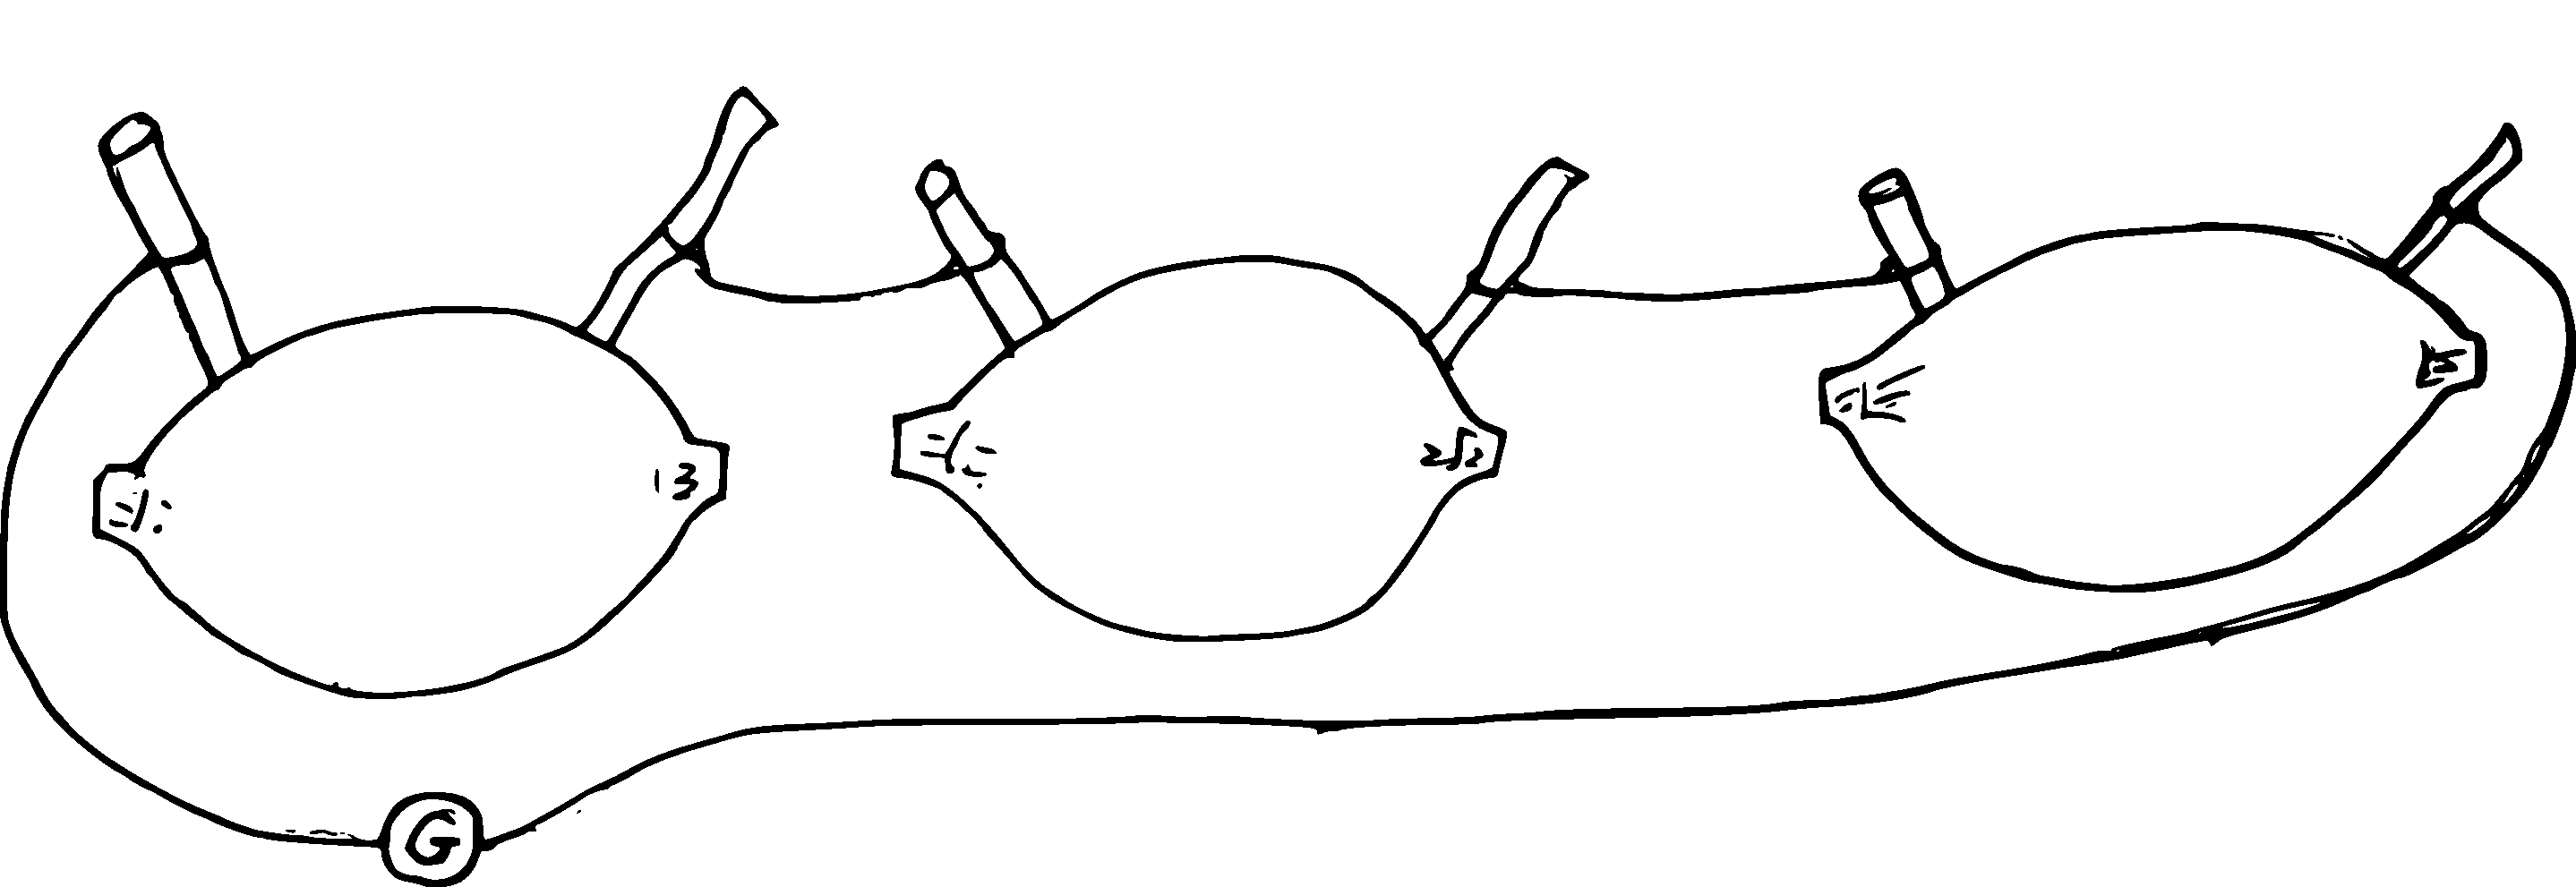
\includegraphics{./img/leclanche-cell.png}
\caption{Building a Leclanche Cell}
\label{fig:leclanche-cell}
\end{center}
\end{figure}

\subsubsection*{Results and Conclusions}
With one lemon connected to the galvanometer a deflection will occur. The deflection will increase with the number of lemons arranged in series. After completing the circuit with enough lemons, the bulb will light up. This shows that a lemon can be used to produce a wet cell known as Leclanche cell.  

\subsubsection*{Clean Up Procedure}
\begin{enumerate}
\item{Collect lemons and throw them in the dust bin. Make sure that people and animals do not eat the used lemons -- they will contain poisonous residual manganese (IV) oxide from the battery and an unhealthy amount of zinc.}
\item{Put other materials in their respective places}
\end{enumerate}

\subsubsection*{Discussion Questions}
\begin{enumerate}
\item{Explain you observations of the completed circuit.}
\item{In the absence of lemons what other materials can be used to create the Leclanche cells?} 
\end{enumerate}

\subsubsection*{Notes}
Electric current can be produced from different sources(cells). There are dry and wet sources of electric cells. Wet cells can be made from natural fruits and foods such as lemon, Irish potatoes and salts which produce electric current based on the principle of Leclanche cells.
